\documentclass[11pt,a4paper]{article}

\usepackage[margin=2cm]{geometry}
\usepackage[T1]{fontenc}
\usepackage{lmodern}
\usepackage{amsmath}
\usepackage{booktabs}
\usepackage{tabularx}
\usepackage{enumitem}
\usepackage{caption}
\usepackage{tikz}
\usetikzlibrary{arrows.meta}

\setlist{itemsep=1pt, topsep=3pt}
\captionsetup{font=small, labelfont=bf}
\setlength{\parskip}{4pt}
\setlength{\parindent}{0pt}

\title{Task 2.4: Signal Chain \& Processing}
\author{Jasper Brinkgreve}
\date{21 October 2026}

\begin{document}
\maketitle

% ---------------------------------------------------------------------------
\section{Scope and design point}

This chain turns the 18 voltage outputs of the $3\times3$ dual-polarisation array into pulse times of
arrival (TOAs) at the worst-case design point. That point is 0.61\,m$^2$ of aperture at 1.2--1.6\,GHz
with an SEFD of about $7.4\times10^{5}$\,Jy. There the pulse peak of J0437$-$4715 lies about 54\,dB
below the receiver noise, and one TOA takes about 20\,h of folding.

The array will go on a ship, so the chain must also follow the ship's motion and tolerate its
transmitters. Nothing in it is tuned for strong signals: each requirement comes from sensitivity,
interference headroom or timing. The digital stages follow the project's validated MATLAB reference
chain (\texttt{processIQ}); the analogue stages and the beamformer are proposed here.

\begin{figure}[ht]
\centering
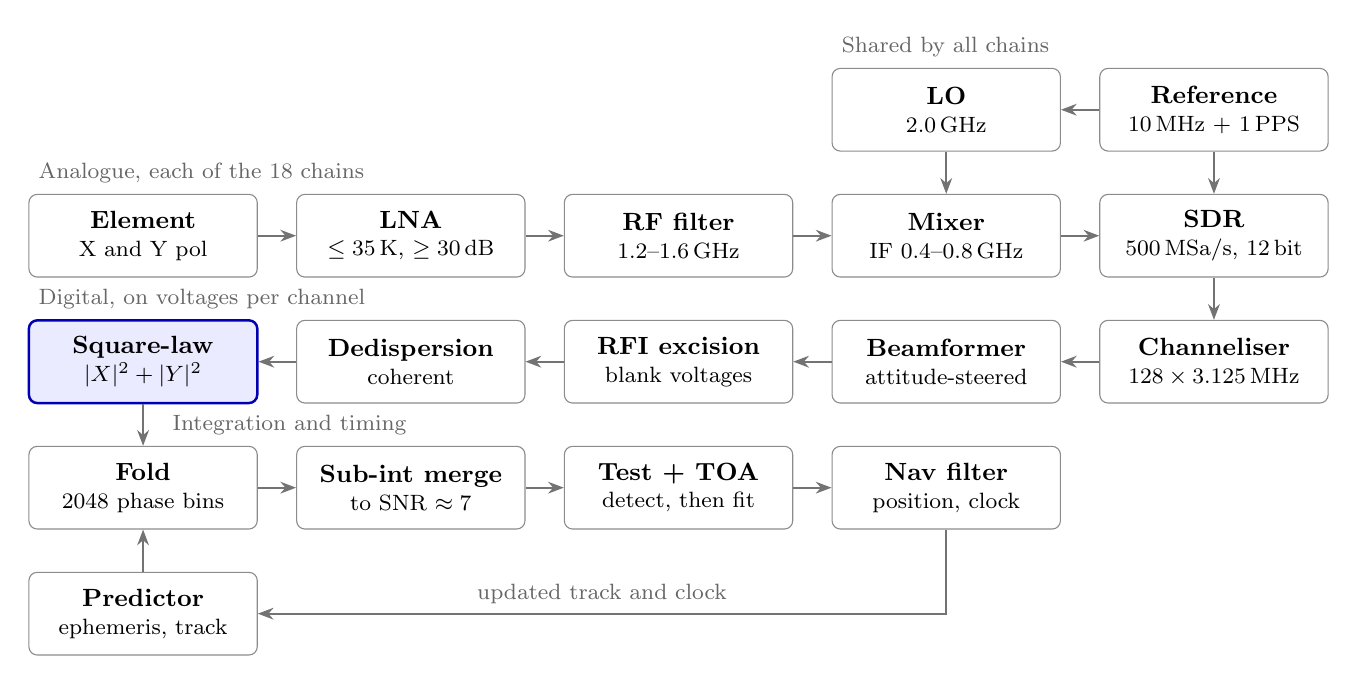
\begin{tikzpicture}[
    blk/.style={draw=black!45, rounded corners=3pt, minimum width=2.9cm, minimum height=1.05cm,
                align=center, font=\small},
    hl/.style={blk, draw=blue!70!black, fill=blue!8, line width=0.9pt},
    arr/.style={-{Stealth[length=2mm]}, draw=black!55, line width=0.6pt},
    lane/.style={anchor=west, font=\footnotesize, text=black!60}]
  \newcommand{\blkt}[2]{\textbf{#1}\\[-1pt]{\footnotesize #2}}

  % row 0: shared LO and reference
  \node[lane] at (8.75, 2.4) {Shared by all chains};
  \node[blk] (lo)  at (10.2, 1.6) {\blkt{LO}{2.0\,GHz}};
  \node[blk] (ref) at (13.6, 1.6) {\blkt{Reference}{10\,MHz + 1\,PPS}};

  % row 1: analogue, left to right
  \node[lane] at (-1.45, 0.8) {Analogue, each of the 18 chains};
  \node[blk] (el)  at (0, 0)    {\blkt{Element}{X and Y pol}};
  \node[blk] (lna) at (3.4, 0)  {\blkt{LNA}{$\le 35$\,K, $\ge 30$\,dB}};
  \node[blk] (bf)  at (6.8, 0)  {\blkt{RF filter}{1.2--1.6\,GHz}};
  \node[blk] (mix) at (10.2, 0) {\blkt{Mixer}{IF 0.4--0.8\,GHz}};
  \node[blk] (sdr) at (13.6, 0) {\blkt{SDR}{500\,MSa/s, 12\,bit}};

  % row 2: digital, on voltages, right to left
  \node[lane] at (-1.45, -0.8) {Digital, on voltages per channel};
  \node[blk] (chan) at (13.6, -1.6) {\blkt{Channeliser}{$128\times3.125$\,MHz}};
  \node[blk] (beam) at (10.2, -1.6) {\blkt{Beamformer}{attitude-steered}};
  \node[blk] (rfi)  at (6.8, -1.6)  {\blkt{RFI excision}{blank voltages}};
  \node[blk] (ded)  at (3.4, -1.6)  {\blkt{Dedispersion}{coherent}};
  \node[hl]  (sq)   at (0, -1.6)    {\blkt{Square-law}{$|X|^2 + |Y|^2$}};

  % row 3: integration and timing, left to right
  \node[lane] at (0.25, -2.4) {Integration and timing};
  \node[blk] (fold)  at (0, -3.2)    {\blkt{Fold}{2048 phase bins}};
  \node[blk] (merge) at (3.4, -3.2)  {\blkt{Sub-int merge}{to SNR $\approx 7$}};
  \node[blk] (toa)   at (6.8, -3.2)  {\blkt{Test + TOA}{detect, then fit}};
  \node[blk] (nav)   at (10.2, -3.2) {\blkt{Nav filter}{position, clock}};

  % row 4: predictor
  \node[blk] (pred) at (0, -4.8) {\blkt{Predictor}{ephemeris, track}};

  \draw[arr] (ref) -- (lo);
  \draw[arr] (ref) -- (sdr);
  \draw[arr] (lo) -- (mix);
  \draw[arr] (el) -- (lna);
  \draw[arr] (lna) -- (bf);
  \draw[arr] (bf) -- (mix);
  \draw[arr] (mix) -- (sdr);
  \draw[arr] (sdr) -- (chan);
  \draw[arr] (chan) -- (beam);
  \draw[arr] (beam) -- (rfi);
  \draw[arr] (rfi) -- (ded);
  \draw[arr] (ded) -- (sq);
  \draw[arr] (sq) -- (fold);
  \draw[arr] (fold) -- (merge);
  \draw[arr] (merge) -- (toa);
  \draw[arr] (toa) -- (nav);
  \draw[arr] (pred) -- (fold);
  \draw[arr] (nav.south) |- node[pos=0.75, above, font=\footnotesize, text=black!60]
      {updated track and clock} (pred.east);
\end{tikzpicture}
\caption{Every phase-sensitive step runs on voltages, before square-law detection. One LO and one
reference serve all 18 chains. The digital row runs right to left; the predictor folds with the
navigation filter's latest track and clock estimate, which closes the loop.}
\label{fig:chain}
\end{figure}

% ---------------------------------------------------------------------------
\section{Front-end receiver}

Each of the 18 outputs (9 elements $\times$ 2 polarisations) has its own LNA, RF filter and mixer, and
one SDR channel digitises the mixer's IF. A single LO, shared by all 18 mixers, keeps the chains
coherent for the beamformer.

\begin{table}[ht]
\centering
\small
\renewcommand{\arraystretch}{1.15}
\begin{tabularx}{\linewidth}{@{}p{2.6cm}XX@{}}
\toprule
Stage & Requirement & Why \\
\midrule
LNA noise & $\le 35$\,K (NF $\le 0.5$\,dB), gain $\ge 30$\,dB, mounted at the feed &
  $T_\mathrm{sys}$ of 60--80\,K must also hold the sky (3--20\,K) and losses; each 0.1\,dB of loss
  before the LNA adds about 7\,K \\
LNA linearity & Set by an RF survey on the ship, not by the pulsar &
  The ship's own Inmarsat uplink (1626.5--1660.5\,MHz) sits 27\,MHz above the band; an en-route radar
  peaks 40\,dB above the noise \\
RF filter, before the mixer & Passband 1.2--1.6\,GHz, ripple $\le 0.5$\,dB; 0.4--0.8 and 2.4--2.8\,GHz
  rejected to below the noise &
  The first band leaks straight through the mixer to the IF, the second is the image; on-board Wi-Fi
  (2.4\,GHz) and LTE (2.6\,GHz) are the likely worst \\
Mixer and LO & High-side LO at 2.0\,GHz, IF 0.4--0.8\,GHz; one LO split to all 18 mixers &
  The LO, its harmonics and its leakage stay outside both the band and the IF; the IF is inverted,
  which the processing must undo \\
LO phase noise & $\le -136$\,dBc/Hz at 3\,MHz offset &
  Reciprocal mixing then spreads a $+40$\,dB radar pulse into the neighbouring channel at least 10\,dB
  below the noise \\
SDR channels & 18 phase-coherent channels, each $\ge 400$\,MHz wide ($\ge 500$\,MSa/s complex) &
  Time per TOA scales as $1/B$, so the full band is worth keeping \\
SDR resolution & $\ge 12$ bits, noise at about 4\,LSB rms &
  Leaves about 50\,dB for a radar pulse before clipping, which would spread RFI into clean channels;
  quantisation loss is negligible (2-bit sampling would cost 12\,\% of the SNR) \\
Sample-clock jitter & $\le 0.2$\,ps rms &
  Jitter noise is $(2\pi f\sigma)^2$ of the input power, $-60$\,dB at the 0.8\,GHz top of the IF: a
  $+40$\,dB radar's jitter noise stays 20\,dB below the receiver noise \\
\bottomrule
\end{tabularx}
\caption{Front-end requirements per analogue chain.}
\label{tab:frontend}
\end{table}

\textbf{If the mixer is the SDR's own.} A built-in quadrature mixer tunes to the band centre, 1.4\,GHz,
because 400\,MHz fills nearly its whole sample rate. Its LO leakage then lands in the protected
1400--1427\,MHz band, and I/Q imbalance mirrors RFI across the centre at $-25$ to $-40$\,dB before
correction. I/Q calibration and blanking of the centre channel then become part of the processing.

\textbf{Pre-processing.} Each SDR's FPGA converts its IF to complex baseband at 500\,MSa/s and splits
it into 128 channels of 3.125\,MHz (a 4/3-oversampled polyphase filterbank). The 18 streams then carry
about 290\,Gbit/s ($18 \times 500$\,MSa/s $\times$ 32\,bit), so the beamformer runs on a GPU server fed
by 100\,GbE links and cuts them to two beams.

\textbf{Local oscillator and timing.} One reference (10\,MHz + 1\,PPS) disciplines the LO synthesiser
and every SDR; the SDRs' own $\pm2$\,ppm crystals are not used. Because one LO feeds all 18 mixers, its
phase noise and drift are common to the chains and drop out of the beam. The SDRs start sampling on the
same PPS edge and count samples from it, so every sample carries a time on the receiver's clock.

That clock's errors enter every TOA. A rate error of $10^{-9}$ builds up 72\,$\mu$s over a 20\,h J0437
fold, six times its 12\,$\mu$s TOA error. B0329+54's 0.5\,ms TOAs tolerate a TCXO; J0437 needs an OCXO
or rubidium reference (4--36\,ns per hour against a TCXO's 3.6\,$\mu$s). The navigation filter carries
clock offset and rate as states, so the design does not depend on GNSS; a GNSS-disciplined reference
serves only as truth during trials.

% ---------------------------------------------------------------------------
\section{Beamforming}

Full digital beamforming, per polarisation and per frequency channel, suits a 9-element array on a ship
best.

\begin{table}[ht]
\centering
\small
\renewcommand{\arraystretch}{1.15}
\begin{tabularx}{\linewidth}{@{}p{4.4cm}cXc@{}}
\toprule
Option & SDR channels & Steering under ship motion & Adaptive nulls per pol. \\
\midrule
Analogue (RF phase shifters) & 2 & Phase steps only; squints across 400\,MHz & None \\
Hybrid (each row of 3 combined in analogue) & 6 & Digital in one axis only & 2 \\
\textbf{Full digital (proposed)} & 18 & True time delay in every channel, updated at $\ge 10$\,Hz & Up to 8 \\
\bottomrule
\end{tabularx}
\caption{Beamforming options for the $3\times3$ dual-polarisation array.}
\label{tab:beam}
\end{table}

\begin{itemize}
\item \textbf{Channels.} The setup already digitises all 18 chains, so a hybrid would save nothing and
  give up nulling and per-element calibration.
\item \textbf{Bandwidth.} The $\sim$0.8\,m aperture delays a wavefront by up to 2.7\,ns, about one cycle
  across 400\,MHz. Weights applied after the channeliser act as true time delay, exact to 0.03\,rad
  within each 3.125\,MHz channel.
\item \textbf{Ship motion.} The steered mount does the slow pointing; a horizontal array would lose
  4.7\,dB at $20^\circ$ elevation. The weights correct the roll and pitch the mount leaves, using the
  ship's attitude sensor, keeping the pulsar within $1.5^\circ$ of the $15^\circ$ beam's centre
  ($\le 0.12$\,dB loss).
\item \textbf{Interference.} Nulls go on the ship's own Inmarsat antenna and on radars near the horizon,
  before temporal excision.
\end{itemize}

\textbf{Calibration.} Each element needs a complex gain per channel, which also absorbs the fixed phase
of its LO path and its SDR. In-band GNSS satellites are point sources at known positions: one satellite
gives about 50\,dB-Hz per element at 70\,K, which fixes each element's phase to well under $1^\circ$ in
seconds. A delay fitted across L2, E6 and L1 (1227.6--1575.42\,MHz) extends this to the whole band.
Between calibrations the chains must stay coherent to about 10\,ps ($6^\circ$ at 1.6\,GHz); $10^\circ$
rms of phase error costs 3\,\% of the array gain.

\textbf{Polarisation.} The X and Y beams are detected and summed as total intensity $|X|^2 + |Y|^2$, so
Faraday rotation and the pulsar's own polarisation drop out.

% ---------------------------------------------------------------------------
\section{Detection and integration pipeline}

At $-54$\,dB no single pulse is visible. The pipeline therefore keeps every phase-sensitive step on
voltages, averages power over hours at a predicted phase, and accepts a TOA only after a formal
detection test. After channelisation and beamforming:

\begin{enumerate}
\item \textbf{Excise RFI on the voltages.} Each channel is searched in windows of 1--16 samples at a
  false-alarm probability of $10^{-6}$, and flagged samples are set to zero. Blanking beats
  subtraction: at $-54$\,dB one radar pulse carries the energy of 80,000 pulsar pulses.
\item \textbf{Dedisperse coherently per channel} to 1.6\,GHz with the catalogue DM. A channel's filter
  stays near 100\,MB at DM 100; one full-band filter would need about 15\,GB.
\item \textbf{Detect.} Square and sum the polarisations, $|X|^2 + |Y|^2$, into 0.96\,$\mu$s bins; the
  data rate falls to about 0.5\,GB/s.
\item \textbf{Fold with a phase predictor} into 2048 phase bins per sub-integration. The predictor turns
  the ephemeris, the ship's dead-reckoned track and the clock estimate into phase polynomials accurate
  to 1\,ns. Without it, Earth's orbital Doppler (up to $10^{-4}$) moves the pulse 12\,ms within a
  120\,s sub-integration.
\item \textbf{Weight channels} by their inverse noise variance, measured off-pulse. The fold also
  weights each bin by the unblanked data it holds.
\item \textbf{Merge sub-integrations adaptively} until each reaches SNR $\approx 7$. In the threshold
  sweep 92\,\% of TOAs were usable at SNR 6 and 100\,\% at SNR 7.5. B0329+54 needs sub-integrations of
  $\le 150$\,s, because its scintillation changes within about 13\,min. J0437's 20\,h TOA spans several
  passes, which the predictor folds together across the gaps.
\item \textbf{Test for detection} (Neyman--Pearson, false-alarm probability $10^{-3}$ per profile). The
  thresholds are $3.09\sigma$ at the predicted phase and $4.15\sigma$ when all phases are searched. A
  TOA is good when the pulse is detected and the profile's $\chi^2$ is not flagged.
\item \textbf{Fit the TOA} by template matching, and pass TOA, error bar and SNR to the navigation
  filter, which solves position and clock.
\end{enumerate}

At the worst-case point, B0329+54 from $52^\circ$\,N reaches SNR 7 in about 3.2\,h, with
$\sigma_\mathrm{TOA} \approx 0.5$\,ms (170\,km). J0437 takes about 20\,h for 12\,$\mu$s (3.6\,km). Time
per TOA scales as SEFD$^2$, so 1\,dB less SEFD saves 37\,\% of the observing time.

% ---------------------------------------------------------------------------
\section{Open points}

\begin{itemize}
\item \textbf{Mixer.} Whether it is a separate downconverter or the SDR's own decides between the two LO
  plans of Section~2.
\item \textbf{Effective area.} The nominal and worst-case points differ by $2.3\times$ in SEFD and
  $5.3\times$ in time per TOA. Most of that is whether 0.61\,m$^2$ is physical or effective.
\item \textbf{Element pitch.} If the nine elements fill 0.61\,m$^2$, they sit about 0.26\,m apart
  ($1.4\lambda$ at 1.6\,GHz), so grating lobes exist. At broadside the element pattern suppresses them;
  steering by $10^\circ$ raises one to roughly $-10$\,dB, so the mount should take most of the motion.
\item \textbf{RF survey on the ship.} The Inmarsat uplink, radar and Wi-Fi levels fix the LNA linearity
  and the filter rejection.
\item \textbf{Oscillator noise.} The reference's Allan deviation over 1--20\,h must be measured on the
  device; datasheets rarely give it.
\end{itemize}

\end{document}
